%Her beskrives kort hvordan projektets HW-dele og SW-dele er implementeret (”lavet”). HW-delene kan med fordel beskrives med få, udvalgte, tydelige fotos. Her beskrives også kort hvordan SW-delene er implementeret (kodet). Den/de anvendte compilere beskrives meget kort (programmeringssprog, version etc.). Der argumenteres for valg af programmeringssprog. Der vises kun source code i projektrapporten, når der er tale om ekstremt interessante, små kodeudsnit. Der henvises til projektets bilag, hvor relevante/tydelige fotos af projektets HW og den samlede source code for projektets SW er anbragt.
\newpage
\chapter{Implementation}
In this section the implementation of Captain system will be discussed. This includes mechanical and electronic hardware choices, as well as software choices.
More detailed descriptions of every thing discussed in this section can be found in the documentation in section~\ref{sec:implementation}, on page~\pageref{sec:implementation}.

\section{Hardware}
There are 2 types of hardware in this project, mechanical and electronic. The mechanics are the boat and rudder and such. The electronics are motor driver, power regulator and so forth.

\subsection{Mechanics}
The mechanics for this project, are the boat saint princess, as seen in figure~\ref{fig:saintprincess}. This boat was chosen simply because it was what was available, and since the project has been rather generic about the choice of hardware up to this point, it doesn't really matter. The boat has a motor in a so call D-drive inboard configuration\cite{motor_config}, which means that the motor is inside the boat and is connected to the propeller via a shaft that goes out through the hull of the boat. The propeller sits just in front of the rudder, which is controlled by a servo on the inside. The hull of the boat is a deep vee hull\cite{hull-types}, it is a planning mode hull, which makes wakes smaller then other hull types.

\begin{figure}[h]
\centering
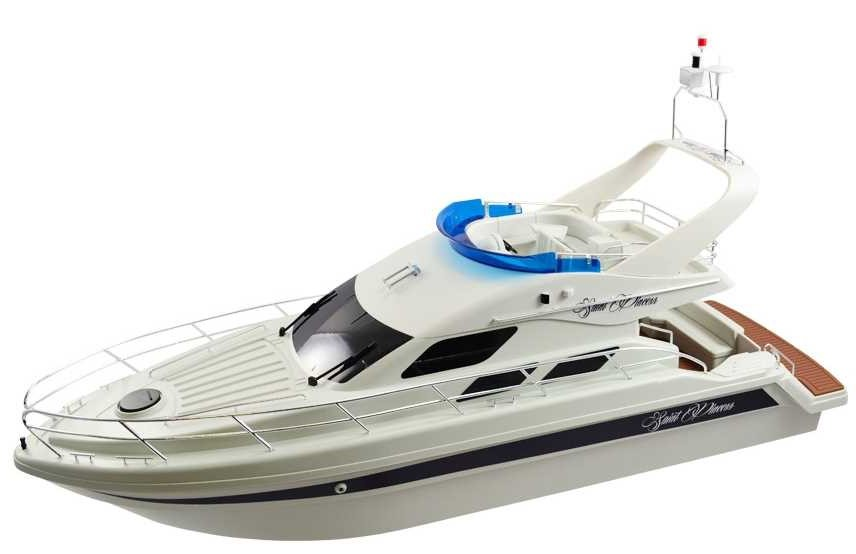
\includegraphics[width=0.7\linewidth]{../Appendix/Project/Dokumentation/Images/Design/saint_princess}
\caption{Saint Princess, a remote controlled yacht\cite{saint_princess}}
\label{fig:saintprincess}
\end{figure}

\subsection{Electronics}
All of the electrical components of the system were connected together on a perfboard. The perfboard is used to distribute the power from the battery to voltage regulators. The signals from the Raspberry pi are also routed through the perfboard, to the servo and the motor controller. All of the signals are routed through detachable wires, to make it easy to measure and rearrange in case some thing was wrong. This perfboard system can be seen in figure~\ref{fig:integration}. 

\begin{figure}[h]
\centering
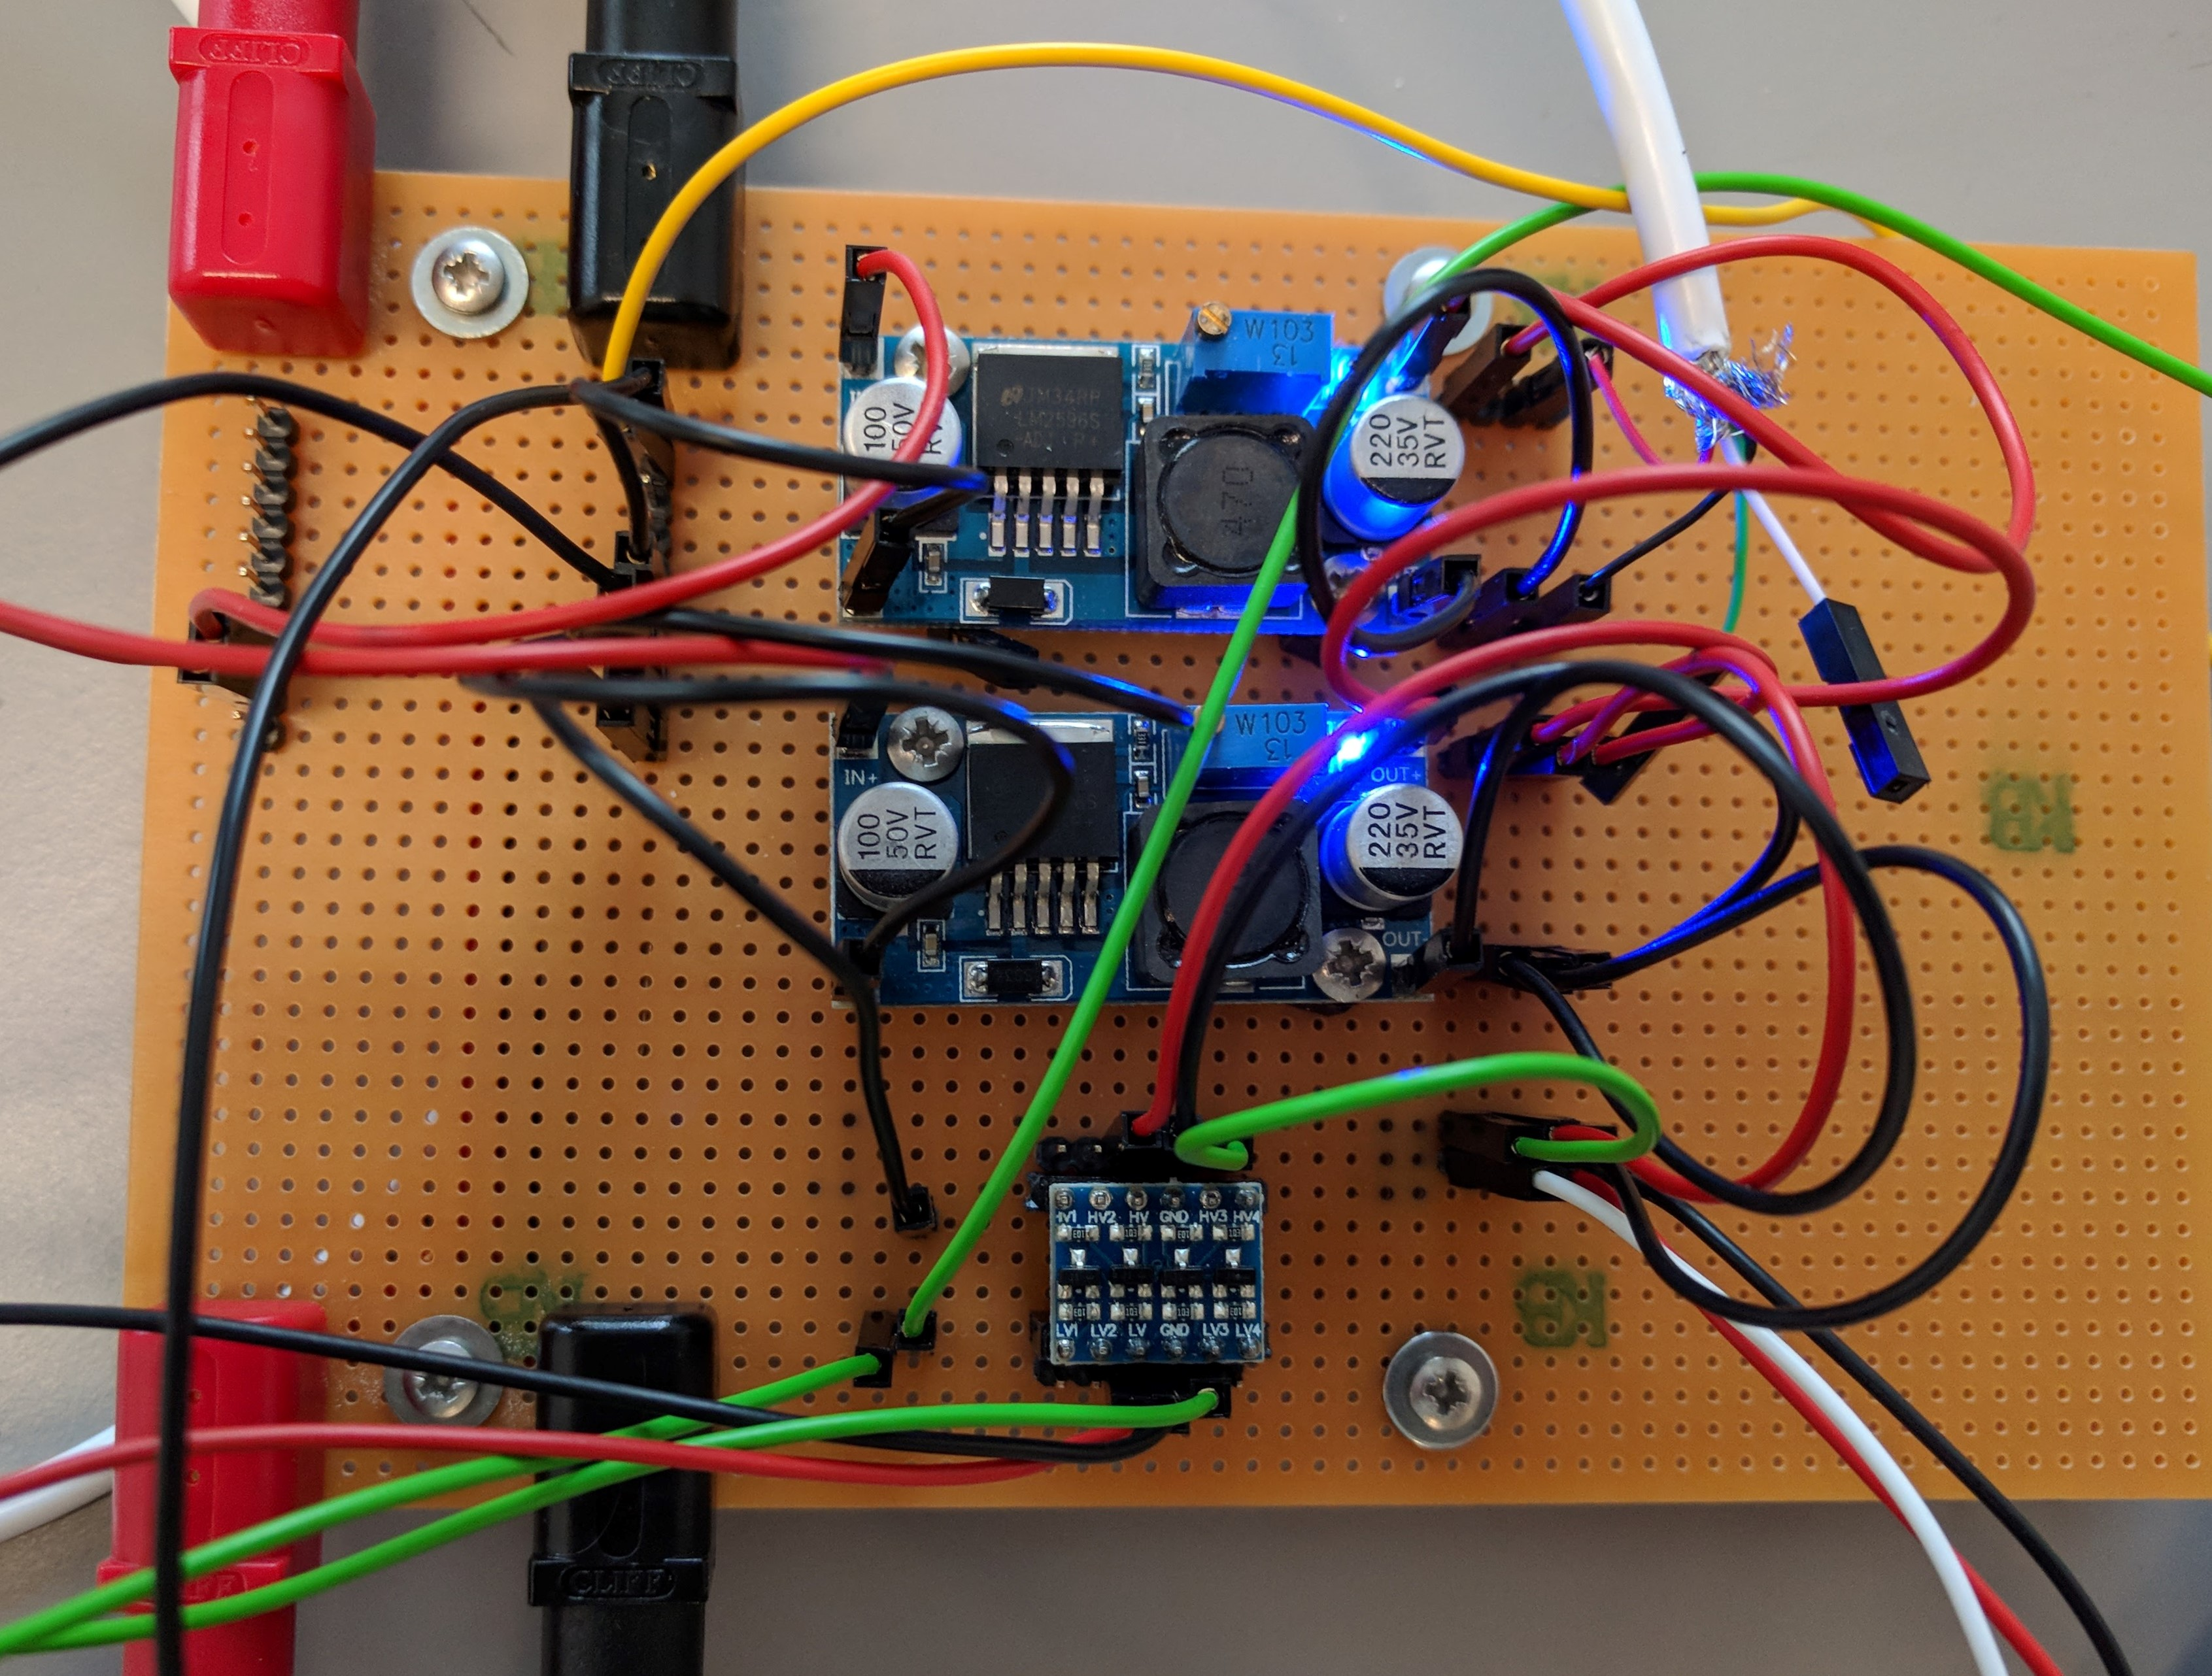
\includegraphics[width=0.7\linewidth]{../Appendix/Project/Dokumentation/Images/Implementation/integration}
\caption{Perfboard, used to connect all components}
\label{fig:integration}
\end{figure}

\section{Software}
In this section, the choices of compilers and programming languages will be discussed. Also the concrete code implementation will be looked at, at a very high level.

\subsection{Programming languages}
This system is built up of 2 distinct parts, at least when discussing software. There is the website user interface, and then there is the controller or what could be thought of as the backend. The website user interface, is marked up in HTML and CSS with the help of a framework called Boostrap~\cite{bootstrap}. In terms of code, javascript was used with AngularJS as a framework. 

Boostrap was chosen simply because it makes it easier to create a website that look somewhat descent. AngularJS was chosen because it makes data binding to the html page very simple, and because it supposedly is a widely used javascript framework.

For the other part of the system, the controller. C++ was the language of choice, this simply because a it is what is familiar. C++ has the advantage of being a very fast. But then the draw back of being a rather low abstraction. 
 
\subsection{Compiler}
For the website there is no real compiler since javascript is an interpreted. But the server that runs the website is a nodejs server. Nodejs is runtime built on the Chrome V8 javascript engine. The client browser used to display the website was a Chrome web browser which is also built on the Chrome V8 javascript engine. 

The controller written in C++ and is therefore compiled, the compiler used while developing the system was the was the VS 2017 C++ Build tools. The compiler used on the Raspberry pi is GCC 6.3.0 for raspbian. They are both C++11 compatible which makes some things easier while developing. 

\subsection{Code}
%To start with lets have a look at the controller code. It is broken up just like the design states. 

One of the key components of the system is the GPS receiver, it is the sole sensor for locating the boat. The controller has a class called Ublox\_neo7m, it is an implementation of the IGPS interface. The Ublox\_neo7m class gets its data by setting up a thread, which continually reads on a serial interface. The data from the serial interface is written to the correct variables. Any other part of the system can get data from the GPS receiver be it, status data like fix and horizontal dilution of precision, or the pose of the boat. 

There are a thruster in the system as well, it is a DC-motor, which can be controlled by a PWM signal. There for the implementation of the class DCMotor uses an object of type IGPIO to send out PWM signals, IGPIO is an interface that describes a general purpose I/O driver for a system. In this case it is for the Raspberry pi and the pigpio library is used\cite{pigpio}. It allows for the motor to set a hardware PWM to a frequency of 30 kHz and a wide spectrum of duty cycles.

As the thruster, the rudder class called Servo, also uses an IGPIO interface to send PWM signals to a GPIO pin. The servo can set the position between 0\% and 100\%. In reality a servos full range of motion is described as period of between 500µS and 2500µS, and a PWM frequency of 50 Hz. So the Servo class converts from one input to the other, it also uses the pigpio built in function called GpioServo. Both the rudder and thruster is in controlled by the autopilot.

The autopilot is in essence built up of two PID loops, one for the rudder, and one for the thruster. In the current implementation, it allows for the user to change the PID terms for the rudder PID loop through the user interface. The autopilots gets the data for what to do from the navigation class.

The Navigation class is TODO!!!! ----- look here!!
%Slut af med The navigation uses the JSONtrasmitter to send data to the userinterface

the ITransmitter interface is implemented as one transmitter a JSONtransmitter, which sends data to the user interface in the form of JSON serialized files. TODO!!!! ----- look here!!
%Slut af med at sende den vidre til recieveren 

To receive data from the user interface, a JSONReceiver has been implemented, as an implementation of the IReceiver interface. The receiver is in change of reading two files that reside in the website. One is the toNav.JSON file, and the other is the activeParam.JSON. toNav.JSON is the file that holds the current command from the website, this could be to calculate a path with a certain rectangle defined. The JSONReceiver then takes this command and data it has been given and passes it on to the navigation through the perform task function. The other file, activeParam.JSON, holds the currently activated parameter profile from the user. The data it gets from this file is passed and then passed on to the appropriate classes, ei either the autopilot or the navigation.

The data that is read or received from the JSONreciever comes from the user interface, which is made up of two parts, a website user interface, that can be opened in the browser, and a nodejs server that host the website. 

The website has four pages, point to point, coverage, status, and edit parameter. The point to point page allows the user to enter one point for the boat to travel to. When the user presses the calculate button, the website sends a POST call to the server hosting it. it sends a command with information about for the calculation to the JSONReceiver. Then it gets a path back from the JSONTransmitter from the fromNav.JSON file, and the path is displayed. The user can now press start, and the start command is send off. Back from the JSONTransmitter comes the progress of completing the path. This sequence is exactly the same for the coverage page, except that it takes two points to calculate. 

The status page on the website has one responsibility and that is parsing the status object that is in the fromNav.JSON file. This object contains diagnostics data for any part of the system. The status page dynamically runs through all of the items and displays them on the screen.

Lastly on the website there is the edit parameter page, this is where the technician setup to boat with all of the changeable parameters. It does this by letting the user create, delete and edit JSON object in a list. This list is saved on the server, along with the currently active parameter profile. 

As mentioned before the user interface also has a nodejs server\cite{nodejs}. It is what is responsible for handling POST calls from the website. All of the POST calls it is setup to handle is for saving data to a file, so both the website and the controller can read it.

%GPS
%Servo / Motor
%Autopilot
%Navigation
%Transmitter
%Reciever
%Hjemme side


%Software
%%compilere
%%Programmeringsprog + argumentation
%%Kode
>>>>>>> b38f97e959aecb20b36bccfcbd75199eacd23e05
